% !TEX root = ../main.tex

\chapter{Background}

In the dynamic landscape of cryptocurrencies, ensuring transparency, accountability, and financial stability
 is paramount for marketplaces. This section provides an overview of the concepts and mechanisms 
 necessary to follow along the conception of a daily proof of liabilities. We explore the various approaches adopted by leading exchanges
  to demonstrate their financial health through proof of reserves or solvency mechanisms. Additionally, we 
  highlight the shortcomings and challenges associated with current solvency verification practices, mainly the lack of recurrent proof of reserves,
   paving the way for a daily proof in the subsequent sections.

\section{Bitcoin}

%Andreas M. Antonopoulos somewhere
Bitcoin is recognized as the world's first successful cryptocurrency and decentralized digital currency. 
The goal of Bitcoin is to allow financial transactions to be settled on its own, without the need of a middleman, typically financial institutions.
Bitcoin is built on a peer-to-peer network, which means that every participant helps in safe keeping the transactions history, and propagating the new transactions.
There is no single point of failure. This allows for transactions to occur in real time, in contrast to the delays encountered in the traditional finance world.
Bitcoin defines two different concepts: Bitcoin the cryptocurrency, and Bitcoin the blockchain. The cryptocurrency resides on the blockchain.
The Bitcoin blockchain is a decentralized ledger that records all Bitcoin (the cryptocurrency) transactions immutably and transparently. 
This blockchain serves as a verifiable record of all Bitcoin transactions, accessible to every participant in the network. 
The transparency afforded by the public blockchain engenders trust and accountability.


\subsection{Transactions}
For every participant of the network, there is a public key, a private key and a wallet address associated with the participant.
The public key is derived from the private key using elliptic curve multiplication, and the wallet address is derived from the public key using a hashing function.
Both are one way function, meaning you cannot derived the other way around.
The public key serves as the unique identifier in the network, but it is the wallet address that typically defines a participant.
The wallet address can be seen as a bank account number. When you send bitcoin to someone, you send it to their wallet address.
To be able to send some bitcoin, you need to create a transaction and send it to the network. 
When transactions are sent on the network, there is no way of knowing who propagated the transaction first.
We need to make sure a transaction originates from the sender. The way to do that is to sign your transaction. The digital signature is created from the transaction data and the private key, which is only known by the owner of the address.
The public key is then used to verify the authenticity of the signature.
Sending a transaction is the easiest problem to solve. The real challenge is to keep track of who owns what, and to avoid the double spending problem.
The methodology for managing this is to keep the history of every single transactions. The transactions are bundled up into blocks, and the chain of blocks create the blockchain.


\subsection{Network}
The challenge of the network, is to have every single node achieve consensus on the transaction history. Nodes are computers connected to the network,
working on publishing new blocks. The nodes work collectively to establish order of transactions (sequencing). Every new transaction is broadcasted to all nodes.
The nodes puts the transactions into a block, and try to publish that block. In order to publish a block, each node needs to solve a proof-of-work challenge.
When a node solves the challenge, it broadcasts the block to every nodes. The nodes accepts the block if all transactions are valid. There is no formal
way of approving a new block. A node show its acceptance by starting to work on a new block using the hash of the accepted block as previous hash.
Some nodes might accept different blocks, if multiple blocks are propagated at the same time. This would create multiple chains. To solve this issue, the longest chain is considered to be the correct one. 
If two chains have the same length, nodes keep working on their respective chains untill one of the chains receives a new block, breaking the tie.


\subsection{Proof-of-work}
In order to submit a new block, a node have to find a hash with a specific number of leading zero bits.
It is exponentially more difficult for every zero bit. 
This cryptographic puzzle serves as a barrier to entry, ensuring that a lot of computational power was spent on creating the block.
The way to test different hash values, is to change the block timestamp, and the nonce value.
The nonce value is there solely for that purpose. Once a block is published, you cannot change any value inside of it because the hash value would change.
The immutability of the older blocks is what makes Bitcoin secure. To modify a block in the middle of the chain, you would need to redo the work of every single blocks made after that.
The longest chain is determined by the cumulative proof-of-work invest in it. This is why we say that Bitcoin is secured as long as 51 pourcent of the nodes are honest.
The chain with the majority of nodes working on it will grow up the fastest, thus will be the accepted chain.
The difficulty of the new block is determined by an average, in order to generate blocks at a steady pace. There is also a bitcoin reward associated with mining (publishing) a block.



\subsection{Merkle Tree}
In the architecture of the blockchain, only the merkle root is stored in the block header. Nodes only keep the recent blocks in memory. For the older blocks, they keep only the block header in memory.
This storage ensures the integrity of the blockchain, while decreasing the memory required to have the full blockchain history.
Since the hash of a block is the hash of the block header, this strategy does not impact the integrity checks of the blockchain.
The merkle root is the top of the Merkle Tree, and is a unique identifier of the full tree. A merkle tree is a tree where the parent node is the hash of the child nodes.
The tree is immutable because changing a single node would have an impact on the merkle root. For instance, in figure 2.1 changing the transaction 0 would change the hash 0,
which in turn would change the hash 01, subsequently changing the root hash.

\begin{figure}[ht!]
\centering
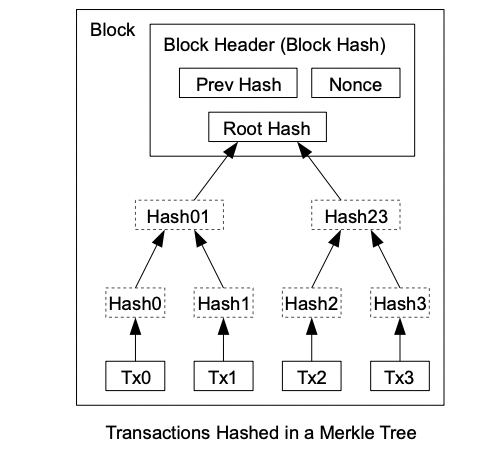
\includegraphics[width=90mm]{MerkleTree.png}
\caption{Bitcoin Merkle Tree \cite{N08}}
\label{overflow}
\end{figure}


\section{Marketplaces}
The best way to buy bitcoin for the first time is through marketplaces. Marketplaces facilitate the exchange of traditional currency for bitcoin.
However, it is crucial to understand that the Bitcoin obtained remain into the custody of the platform, rather than being deposited to a personal wallet address.
In order to gain custody of your bitcoins in your wallet, you need to enter a transfer request. This is similar to traditional finance, where you trust the bank (marketplace), to
go ahead with your transaction. Once you have bitcoins in your wallet, you can transact on the network without needing a 3rd party.
Unless you are running a node, you will need to trust a 3rd party, whether it is a marketplace, or over the counter, to first acquire bitcoin.

When the bitcoin you own is in custody of the marketplace, there is no way to see your bitcoin onchain. Marketplaces have many wallets, some are made public and some are not.
While this allo for the privacy of your marketplace deposits and withdraws, it represent an fondamental contradiction. Bitcoin was designed to be transparent and public, without the need of a 3rd party to do a transaction.
Not being able to track your bitcoin in the marketplace pauses a significant challenge. A user has no proof that the marketplace solvency to reimburse
every client. 
However, this problem is being actively worked on. Marketplaces have begin to use proof of solvency (or proof of reserve) to demonstrate that they are solvent.
While this is a step in the right direction, the current proof of solvency used by the marketplaces have many default, and they are not sufficient to prove that they are solvent.
%Talk about FTX


\section{Zero Knowledge}

Zero-knowledge proofs is a cryptographic technique to prove some knowledge without divulging any informations.For instance,
the classic way of proving that you know the solution to an equation, is to reveal the solution to the equation itself.
However, with zero knowledge you are able to prove that you know the solution, without discolsing the solution. 
To construct a zero knowledge proof, you need to construct a proof that is sound and complete. You also need your proof to be zero knowledge\cite{LZK}.

\begin{itemize}

    \item \textbf{Completeness}: If the statement is true, an honest verifier will be convinced by an honest prover.
    
    \item \textbf{Soundness}: If the statement is false, no dishonest prover can convince the honest verifier (except with some infinitysimal probability).
    
    \item \textbf{Zero-Knowledge}: If the statement is true,  a verifier learns nothing other than the fact that the statement is true. \cite{LC23}
    
    \end{itemize}

    \subsection{Non interactive proofs} 



Zero knowledge proofs were originally designed as interactive, that is multiple rounds of interaction between the prover and the verifier \cite{GMR89}.
 leading to what are called interactive zero-knowledge proofs. This interaction allows the prover to demonstrate knowledge of the solution without revealing any additional information.
 An alternative model was then proposed where the verifier and prover use a reference string that is shared during a trusted setup. Once we have the reference string, a single message is needed between the prover and the verifier.
 The elimination of multiple rounds of interaction simplifies the verification process and reduces the computational power required. 
 Therefore, noninteractive zero-knowledge proofs offer enhanced efficiency and scalability, which will be needed later on.  \cite{BFM88} \cite{GMW91}


 \subsection{SNARKS} 
One of the recent advancement for non-interactive proofs is what is known as SNARK (non-interactive argument of knowledge).
This means a proof that is:
\begin{itemize}

    \item \textbf{Succinct}: the size of the proof is very small compared to the size of the witness.
    
    \item \textbf{Non-interactive}: No rounds of interactions between the prover and the verifier.

    \item \textbf{Argument}: Secured only for provers with bounded computational ressources, that is a dishonest prover with unlimited computational power could prove a wrong statement.

    \item \textbf{Knowledge-sound}: If the statement is true,  a verifier learns nothing other than the fact that the statement is true. \cite{NZ20}
    
    \end{itemize}

Moreover, a SNARK can also be zero-knowedge, where the prover demonstrate knowledge without revealing any additional information about the witness. We call such proof a zk-SNARK.

\subsection{Arithmetic circuit} 



Arithmetic circuits are a core component of SNARKS. An arithmetic circuit is a set gates, each assigned a distinct set of inputs corresponding to the numbers to be processed in the operation. 
These gates are configured to execute arithmetic operations such as addition, subtraction, multiplication, or division. The outputs of the gate circuit represent the digits of the resulting computation.
This structure allows SNARKs to efficiently verify complex mathematical computations while preserving succinctness and scalability.

\begin{figure}[H]
    \centering
    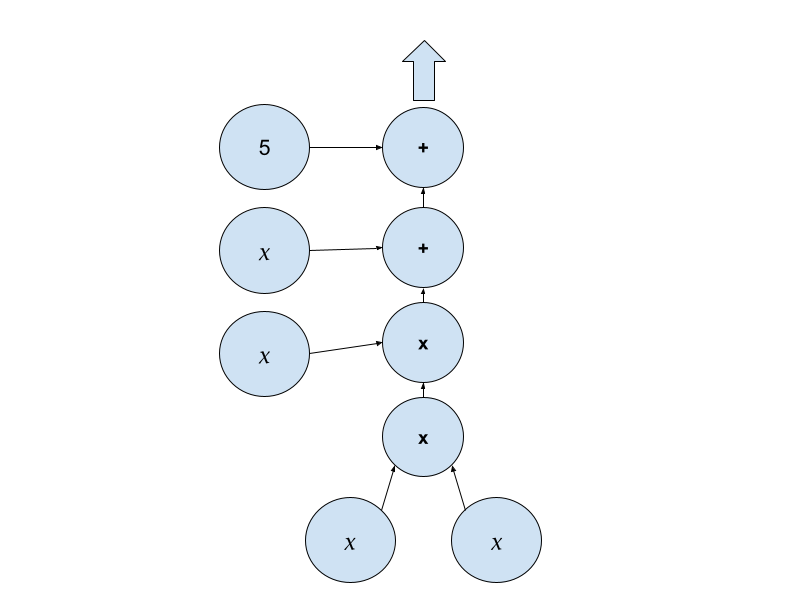
\includegraphics[width=60mm]{ArithmeticCircuit.png}
    \caption{General Arithmetic circuit \cite{ZKM2}}
    \label{overflow}
    \end{figure}



The prover's process in SNARKs is to create a proof using the setup parameter, a private witness, and public input. The proof shows that the arithmetic circuit is equal to 0. 
Using the same setup parameter and the public input, the verifier confirms the accuracy of the proof by making sure it aligns with the parameters.

\begin{figure}[H]
    \centering
    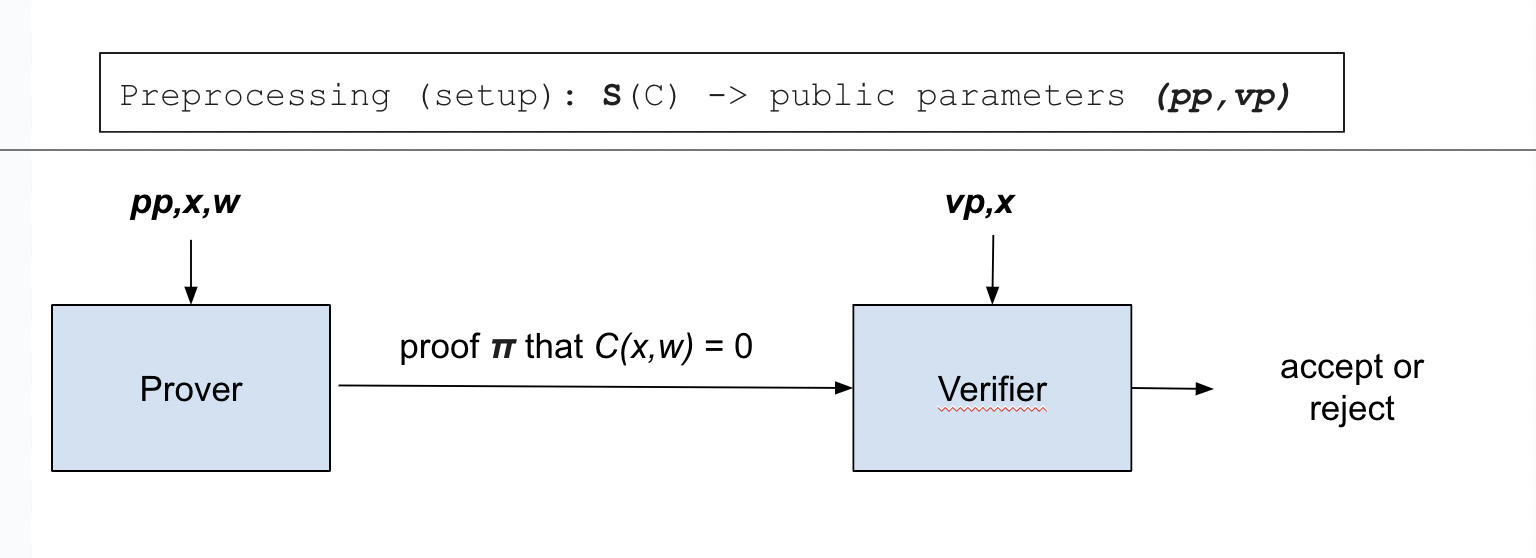
\includegraphics[width=130mm]{Circuit.png}
    \caption{Arithmetic circuit for SNARK \cite{ZKM2}}
    \label{overflow}
    \end{figure}

\begin{itemize}

    \item \textbf{S(C)}: Public parameters (pp,vp) for prover and verifier
    
    \item \textbf{P(pp,x,w)}: Proof $\pi$

    \item \textbf{V(vp,x,$\pi$)}: Accept or reject

    \item \textbf{C(x,w)}: Arithmetic circuit

    \item \textbf{w}: Private witness

    \item \textbf{x}: Public input
    
    \end{itemize}

%If STARK is mentionned later, define it here



\section{Proof of solvency}

A proof of solvency is a system where we prove that an entity, in most cases an exchange, hold enough assets to cover
the balance of every customers. In traditional finance, this would be done thourgh an audit. While an audit can be usefell,
it has many limitations. Obviously it requires the trust of another 3rd party, but it poses also a time constraint. Thus, it is impractical, even impossible
to hold an audit every single day, and in the bitcoin world things move fast. It is essential to be able to fill a prove of solvency every single day.
The implementation of a mechanism to produce daily proofs of solvency is therefore of the utmost importance.

A proof of solvency is composed by a proof of assets, where we verify what assets the marketplace as control over, and the proof of liabilities,
where we confirm that the total amount of user deposits is smaller than the marketplaces assets. 


The first paper about a proof of solvency focuses only on the proof of liabilities. In his paper Gregory Maxwell addresses the issue of verifying 
the solvency of Bitcoin exchanges. \cite{chainlink_blog}
Maxwell's system ensures user privacy by maintaining confidentiality of individual account balances, while only revealing aggregate information in the proof of liabilities. 
This is achieved through the application of Merkle trees. 

\begin{figure}[H]
    \centering
    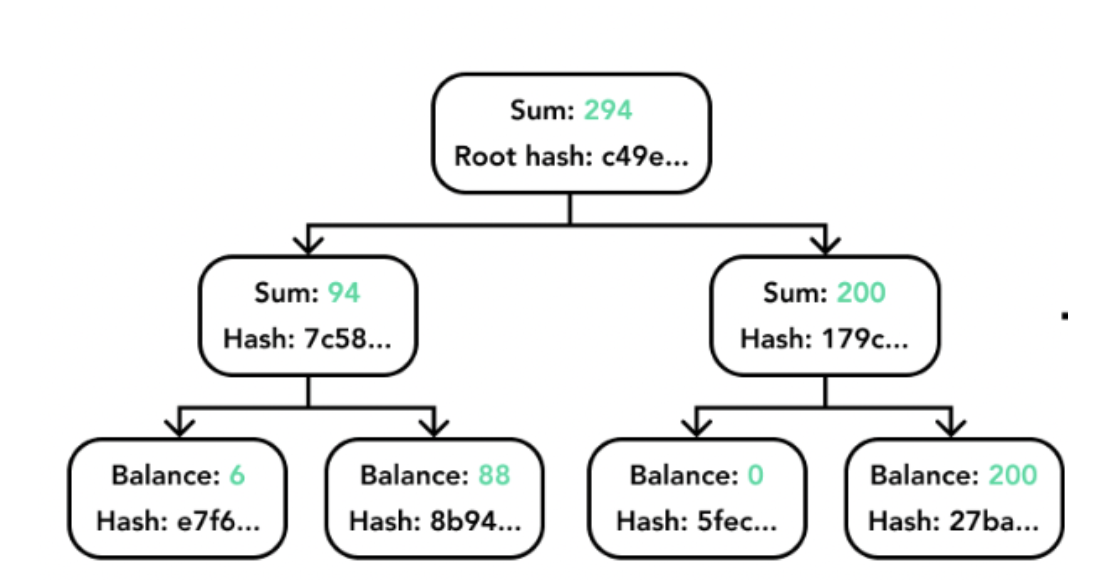
\includegraphics[width=130mm]{MerkleTreeLiabilities.png}
    \caption{Merkle tree for proof of liabilities}
    \label{overflow}
    \end{figure}

In the Merkle tree, every node contains a user's balance along with a hash-based commitment incorporating the customer ID and a nonce. The root of the tree is the sum of the balances. 
To verify their inclusion in the total liabilities, users receive a subset of the hash tree from the exchange. This subset includes the user's nonce and the sibling nodes along the unique path from the user's leaf node to the root. 
By comparing the received information to the exchange's broadcasted root node, users can confirm the inclusion of their balance.
While elegant, the protocol does have privacy implications. The exact value of the exchange's total liabilities, published in the root node, may be sensitive data. 
Additionally, the proof of inclusion reveals the neighbor's balance, and the subtree's balance along the Merkle path. 

The proof of liabilities is only part of the proof of solvency. A complete proof of solvency needs a proof of asset as well.
Provision describes the first preserving privacy proof of asset \cite{DBBBCC15}.

In Provisions, the focus shifts towards preserving privacy while still proving ownership of assets. 
Instead of publicly demonstrating control over specific addresses, Provisions enables exchanges to prove ownership of an anonymous subset of addresses sourced from the blockchain.

Since these 2 papers, a lot of work was done to make the proof of solvency evolve. However, marketplaces still do not implement a proof of solvency, or a flawed and limited version of it.


\subsection{Real world proof of solvency} 
In recent years, several major cryptocurrency exchanges, including Binance, Crypto.com, and Kraken, have taken steps to enhance transparency by provinding various proof of reserves.
Binance has implemented a proof of reserves system where they publish a monthly Merkle tree as their proof of liabilities, and disclose a list of their assets \cite{BPR}. 
Crypto.com published a one-time audit \cite{CC22}. 
Kraken is also publishing a proof of liabilities every few months, without a proof of assets. \cite{KK23}.

Although these proof of reserves may seem promising initially, they are primarily superficial.
The proofs have many shortcomings, they are not sufficient to prove that the marketplaces are solvent.
The first concern is the lack of proof of assets, or in Binance's case the lack of evidence demonstrating control over the wallets.
Without a reliable proof of assets, the proof of liabilities is worthless because it has nothing to compare against.

Moreover, the frequency of reporting is another area of concern. Given the dynamic nature of cryptocurrencies, a monthly report is not sufficient at all.
Binance is the only marketplace describing their proof of solvancy, and we can see that it is not built with recurrence in mind.
The proof is created from scrach every time. They would need 150 servers to produce a daily proof \cite{BPS}.




 



